\chapter{Diferenciação celular: a célula muscular esquelética}\label{ch:b2:cell-differentiation}

Uma fibra do músculo da sua coxa é uma única célula de trinta
centímetros de comprimento, com centenas de núcleos, repleta de uma
ponta à outra de bastões contráteis tão regulares que ela parece
listrada ao microscópio. Ela começou como um aglomerado de células de
aparência comum que saíram de um somito, se multiplicaram, pararam de
se dividir, se alinharam, se fundiram e ativaram várias centenas de
genes que nunca tinham usado. Todas as células do corpo têm o mesmo
genoma; uma \omterm{def:b2:cell-differentiation:myogenesis}{fibra muscular} é o que esse genoma faz quando um \omterm{prop:b2:cell-differentiation:transcriptional}{fator de
transcrição} específico é ativado. Este capítulo toma a célula muscular
esquelética como exemplo resolvido da \emph{\omterm{def:b2:cell-differentiation:differentiation}{diferenciação}} --- como uma
célula adquire e conserva uma identidade especializada ---, e a célula
muscular é um bom exemplo porque o interruptor mestre é conhecido, as
etapas podem ser observadas numa placa de cultura e a célula acabada é
uma máquina cujas peças são visíveis.

\section{O que é a diferenciação}

\begin{definition}[Diferenciação, determinação, potência]\label{def:b2:cell-differentiation:differentiation}
\index{diferenciação}\index{determinação}\index{célula-tronco}\index{potência}
Uma célula está \emph{diferenciada} quando expressa o padrão estável
de genes --- e portanto as proteínas, a forma e a função --- de um tipo
celular. Ela está \emph{determinada} (ou comprometida) quando seu
destino está fixado embora sua diferenciação ainda não tenha começado:
um \omterm{def:b2:cell-differentiation:myogenesis}{mioblasto} se parece com um fibroblasto, mas só formará músculo. A
\emph{potência} é o leque de tipos que uma célula ainda pode originar:
\emph{totipotente} (o zigoto e os primeiros blastômeros, que formam
tudo, inclusive a \omterm{def:b2:mammal-reproduction:placenta}{placenta}), \emph{pluripotente} (a \omterm{def:b2:mammal-reproduction:implantation}{massa celular
interna}, que forma todos os tecidos do corpo), \emph{multipotente}
(uma célula-tronco do sangue ou do músculo, que forma os tipos de um
tecido), \emph{unipotente}. Uma \emph{célula-tronco} é uma célula que
se divide dando uma filha igual a ela e outra que segue para a
diferenciação, o que mantém o estoque enquanto abastece o tecido. Na
maioria dos casos, a diferenciação não é uma perda de genes, mas uma
escolha entre eles: o genoma de um núcleo muscular está completo.
\end{definition}
\begin{proof}[Evidências]
Gurdon (1962) transplantou o núcleo de uma célula intestinal
diferenciada de um girino para um ovo de rã cujo próprio núcleo fora
destruído; uma fração dos ovos se desenvolveu em rãs normais e
férteis. O núcleo diferenciado não tinha perdido nenhum dos genes
necessários para formar um animal inteiro; o citoplasma do ovo o
reiniciara. A mesma operação com o núcleo de uma célula mamária num
óvulo de ovelha deu Dolly (1996), e a reprogramação de um fibroblasto
da pele numa \omterm{def:b2:cell-differentiation:differentiation}{célula-tronco} pluripotente por quatro \omterm{prop:b2:cell-differentiation:transcriptional}{fatores de
transcrição} (Yamanaka, 2006) mostrou que a reinicialização pode ser
feita com um punhado de proteínas.
\end{proof}

\begin{proposition}[A diferenciação é transcricional]\label{prop:b2:cell-differentiation:transcriptional}
\index{fator de transcrição}\index{regulador mestre}
A diferença entre dois tipos celulares está nos genes que são
transcritos. Alguns \emph{\omterm{prop:b2:cell-differentiation:transcriptional}{fatores de transcrição}}, expressos em
resposta aos sinais indutores do \cref{ch:b2:vertebrate-development}, ligam-se às regiões
reguladoras de centenas de genes-alvo e os ativam, enquanto os genes
de outros destinos são desligados; e, como um fator desse tipo
costuma ativar o próprio gene, o estado, uma vez alcançado, se
autossustenta. Para alguns tecidos, um único fator é um
\emph{\omterm{prop:b2:cell-differentiation:transcriptional}{regulador mestre}}, suficiente para impor o destino a uma célula
de outro tipo: \omterm{def:b2:cell-differentiation:myogenesis}{MyoD} para o músculo esquelético, Pax6 para o olho, Sox9
para a cartilagem. O estado é estabilizado ainda mais por mudanças na
cromatina --- metilação do DNA, modificação das histonas --- que mantêm
silenciados os genes silenciados ao longo das divisões (a
\emph{epigenética} do volume do Ano 3). Uma célula diferenciada
lembra, portanto, o que ela é sem nenhuma mudança em sua sequência de
DNA, e essa memória está escrita no padrão de fatores e de cromatina,
e não nos genes.
\end{proposition}

\section{A formação de uma fibra muscular}

\begin{definition}[Miogênese]\label{def:b2:cell-differentiation:myogenesis}
\index{mioblasto}\index{miotubo}\index{fibra muscular}\index{MyoD}
No embrião, células do dermomiótomo do somito são induzidas por sinais
do \omterm{prop:b2:vertebrate-development:neurulation}{tubo neural}, da notocorda e do ectoderma superficial a expressar os
fatores miogênicos \emph{MyoD} e \emph{Myf5}: elas são agora
\emph{mioblastos}, determinados, mas ainda em divisão e de aparência
banal. Os mioblastos migram --- para os \omterm{def:b2:limb-organogenesis:bud}{brotos dos membros}, por exemplo
--- e se multiplicam enquanto houver fatores de crescimento (FGF).
Quando esses fatores se esgotam, eles saem do ciclo celular, expressam
um segundo fator, a \emph{miogenina}, alinham-se pelas extremidades e
se \emph{fundem}: suas membranas se unem num único \emph{miotubo}
longo, com muitos núcleos em fila. O miotubo ativa os genes musculares
--- actina, miosina, troponina, tropomiosina, creatina-quinase, o
receptor de acetilcolina ---, monta o aparelho contrátil e amadurece
numa \emph{fibra muscular}, cujos núcleos ficam na periferia. Uma fibra
nunca mais se divide; alguns mioblastos permanecem ao lado dela,
quiescentes, como \emph{células satélites}, as \omterm{def:b2:cell-differentiation:differentiation}{células-tronco} que
reparam o músculo e o fazem crescer por toda a vida.
\end{definition}

\begin{omfigure}
\begin{tikzpicture}[every node/.style={font=\scriptsize}, >=stealth]
  % somite
  \draw[thick, fill=omProp!25] (0,0) ellipse (0.6 and 0.5); \node[below, align=center] at (0,-0.6) {somito\\(dermomiótomo)};
  \draw[->, thick] (0.7,0) -- (1.6,0) node[midway, above=0.35cm, align=center] {indução\\Wnt, Shh};
  % myoblasts dividing
  \foreach \p in {(2.2,0.3),(2.7,-0.3),(3.2,0.3),(3.7,-0.3)} \draw[thick, fill=omDef!25] \p ellipse (0.28 and 0.18);
  \node[below, align=center] at (3.0,-0.6) {mioblastos: MyoD, Myf5\\dividem-se enquanto há FGF};
  \draw[->, thick] (4.1,0) -- (5.0,0) node[midway, above=0.45cm, align=center] {FGF retirado:\\miogenina,\\saída do ciclo};
  % aligned, fusing
  \foreach \x in {5.35,5.95,6.55,7.15} \draw[thick, fill=omDef!25] (\x,0) ellipse (0.3 and 0.16);
  \node[below, align=center] at (6.25,-0.6) {alinhamento e fusão};
  \draw[->, thick] (7.6,0) -- (8.5,0);
  % myotube
  \draw[thick, fill=omDef!15, rounded corners=6pt] (8.7,-0.3) rectangle (12.6,0.3);
  \foreach \x in {9.2,10.0,10.8,11.6,12.3} \fill[omDef!80!black] (\x,0) ellipse (0.13 and 0.08);
  \node[below, align=center] at (10.65,-0.6) {miotubo: muitos núcleos,\\genes musculares ativos, miofibrilas montadas};
\end{tikzpicture}

{\small A miogênese: células induzidas do somito se tornam \omterm{def:b2:cell-differentiation:myogenesis}{mioblastos}
em divisão; quando os fatores de crescimento são retirados, eles param
de se dividir, alinham-se e se fundem num \omterm{def:b2:cell-differentiation:myogenesis}{miotubo} multinucleado que
ativa os genes musculares.}
\end{omfigure}

\begin{omfigure}
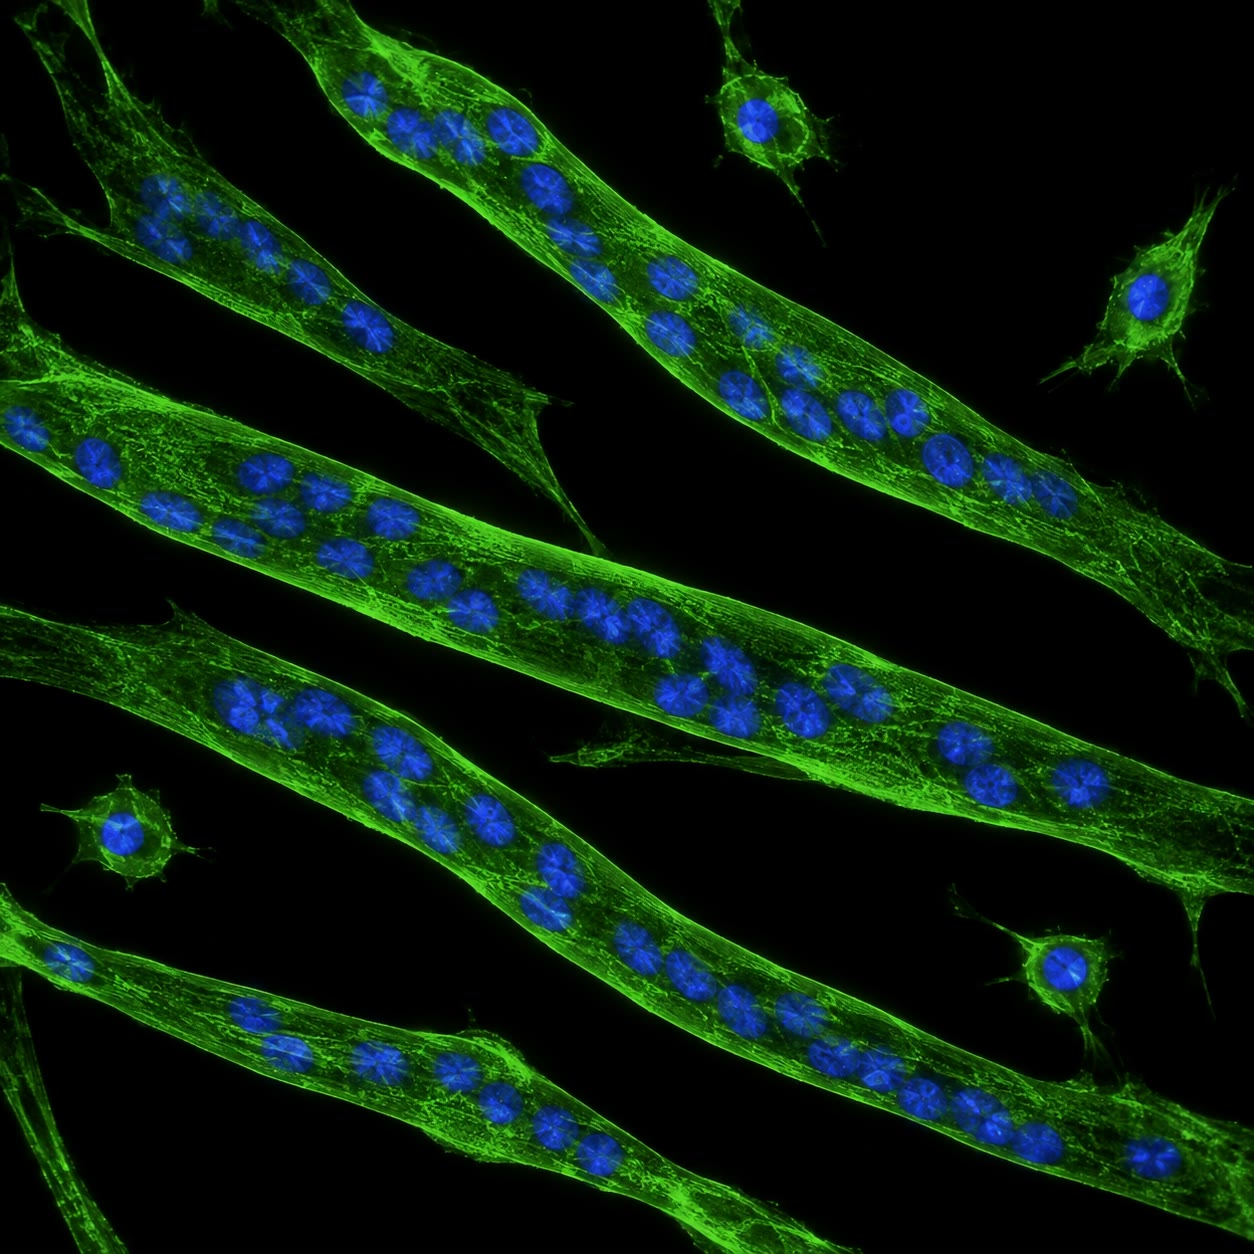
\includegraphics[width=0.44\linewidth]{images/book4/ai/b4-12-myotubes.jpg}\hspace{0.04\linewidth}
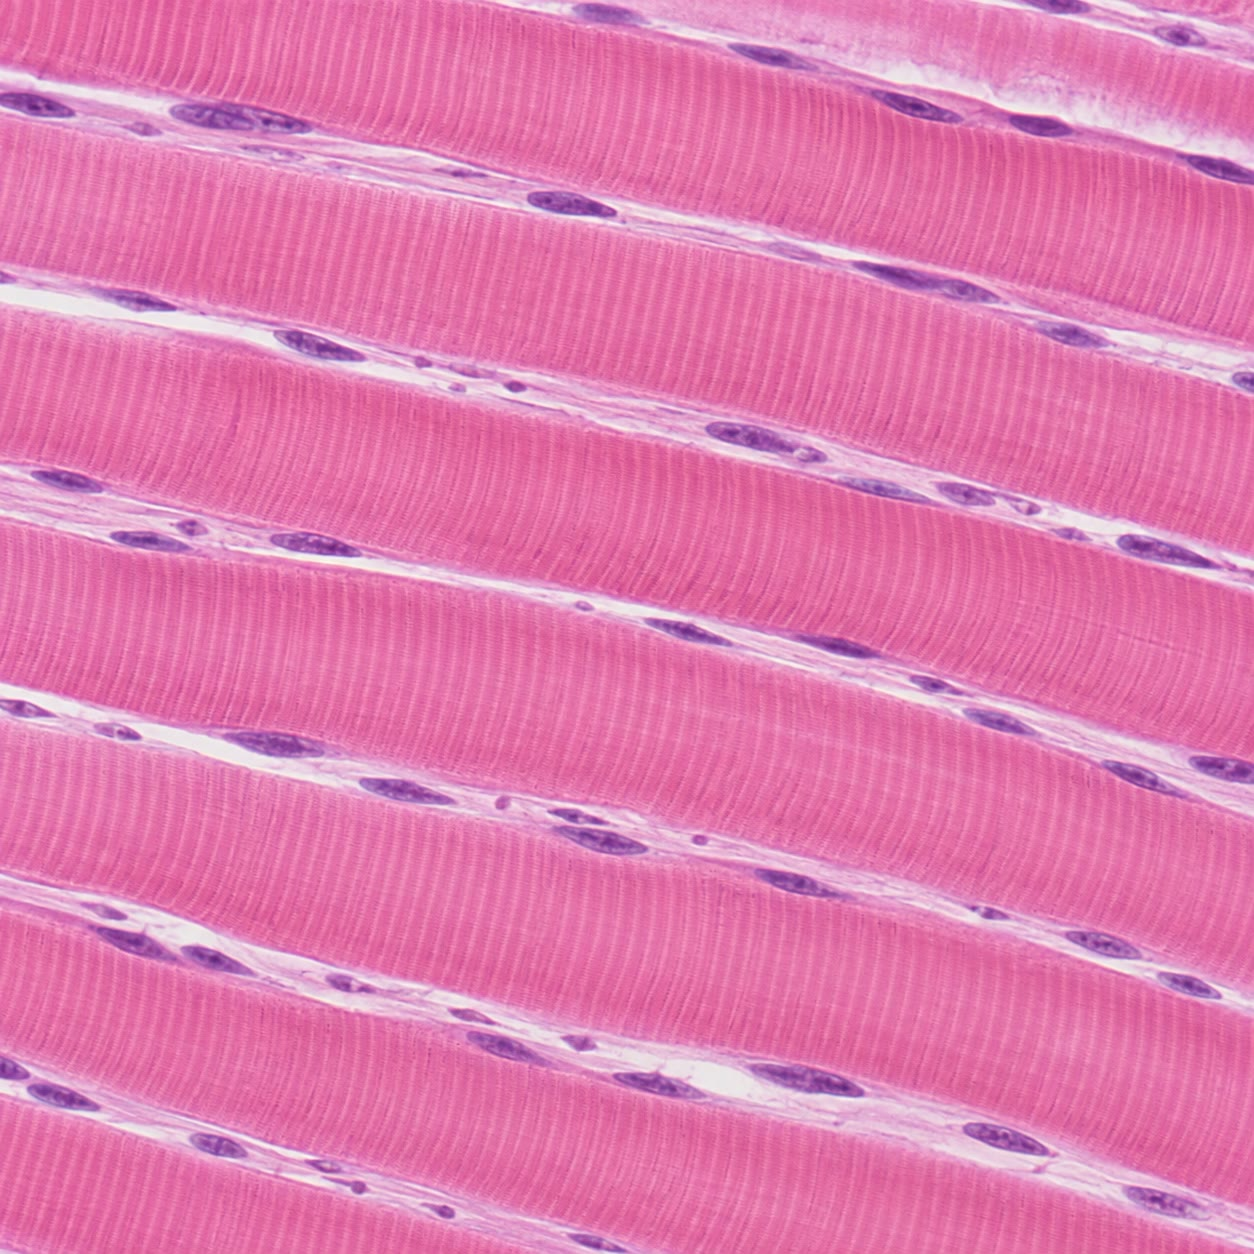
\includegraphics[width=0.44\linewidth]{images/book4/ai/b4-12-muscle-fibres.jpg}

{\small À esquerda: \omterm{def:b2:cell-differentiation:myogenesis}{miotubos} em cultura, cada um uma célula fundida com
uma fileira de núcleos, ao lado de \omterm{def:b2:cell-differentiation:myogenesis}{mioblastos} isolados que ainda não se
fundiram. À direita: fibras maduras em vista longitudinal, com suas
estriações transversais formadas pelos \omterm{def:b2:cell-differentiation:fibre}{sarcômeros} repetidos e seus
núcleos empurrados para a borda.}
\end{omfigure}

\begin{proposition}[MyoD: um interruptor mestre]\label{prop:b2:cell-differentiation:myod}
\index{regulador mestre!MyoD}
A \omterm{def:b2:cell-differentiation:myogenesis}{MyoD} é um \omterm{prop:b2:cell-differentiation:transcriptional}{fator de transcrição} da família hélice-alça-hélice. Ela se
liga, como dímero com uma proteína parceira ubíqua, a uma sequência de
seis bases (o E-box, CANNTG) nas regiões reguladoras dos genes
musculares, recruta enzimas que abrem a cromatina e ativa os genes ---
inclusive os genes da miogenina e da própria \omterm{def:b2:cell-differentiation:myogenesis}{MyoD}, e é assim que o
estado se mantém. Sua atividade é controlada: nos \omterm{def:b2:cell-differentiation:myogenesis}{mioblastos} em
divisão, uma proteína inibidora (Id), induzida pelos fatores de
crescimento, sequestra a parceira e mantém a \omterm{def:b2:cell-differentiation:myogenesis}{MyoD} inativa; quando os
fatores de crescimento são retirados, a Id desaparece e a \omterm{def:b2:cell-differentiation:myogenesis}{MyoD} age.
Como a \omterm{def:b2:cell-differentiation:myogenesis}{MyoD} basta para impor o programa muscular a um fibroblasto, a
uma célula adiposa ou a uma célula nervosa, o destino muscular está, em
certo sentido, a um gene de distância: a dificuldade de se tornar
músculo não está em saber como, mas em receber a ordem.
\end{proposition}
\begin{proof}[Evidências]
Davis, Weintraub e Lassar (1987) transferiram um único cDNA, isolado de
\omterm{def:b2:cell-differentiation:myogenesis}{mioblastos}, para fibroblastos em cultura: os fibroblastos pararam de se
dividir, fundiram-se em \omterm{def:b2:cell-differentiation:myogenesis}{miotubos} e produziram proteínas musculares. O
gene recebeu o nome de \omterm{def:b2:cell-differentiation:myogenesis}{MyoD}. Seus parentes Myf5, miogenina e MRF4
foram encontrados por homologia; um camundongo sem \omterm{def:b2:cell-differentiation:myogenesis}{MyoD} e sem Myf5 não
tem \omterm{def:b2:cell-differentiation:myogenesis}{mioblastos} nem músculo esquelético algum, ao passo que um
camundongo sem miogenina tem \omterm{def:b2:cell-differentiation:myogenesis}{mioblastos} que nunca se fundem.
\end{proof}

\begin{theorem}[Um interruptor autossustentado]\label{thm:b2:cell-differentiation:switch}
\index{biestabilidade}\index{retroalimentação positiva!gênica}
Seja $m$ a quantidade de um fator que ativa o próprio gene com uma
resposta cooperativa (sigmoide) e é degradado à taxa $k$:
\[
\frac{\mathrm{d}m}{\mathrm{d}t} = \frac{a\,m^{2}}{K^{2} + m^{2}} + b - k\,m,
\]
em que $b$ é uma pequena síntese basal. Para valores adequados de $a$,
$b$, $K$ e $k$, essa equação tem \emph{dois} estados estacionários
estáveis, um baixo, perto de $b/k$, e um alto, perto de $a/k$,
separados por um limiar instável: a célula é \emph{biestável}. Um sinal
indutor transitório que empurra $m$ acima do limiar leva a célula ao
estado alto, onde ela permanece depois que o sinal desaparece; abaixo
do limiar, ela volta ao estado baixo. É uma memória construída a
partir de uma alça de retroalimentação, e é por isso que uma célula,
uma vez comprometida, permanece comprometida ao longo das divisões e na
ausência do indutor.
\end{theorem}
\begin{proof}
Os estados estacionários satisfazem $k m = a m^{2}/(K^{2} + m^{2}) + b$.
O lado direito é uma sigmoide que sobe de $b$ a $a + b$; o esquerdo é
uma reta pela origem, de inclinação $k$. Para $b/k < K$ e $k$ pequeno o
bastante para que a reta corte a parte íngreme da sigmoide, as duas
curvas se cruzam três vezes: em $m_{\text{baixo}} \approx b/k$, num
valor intermediário $m_{\text{u}}$ e em $m_{\text{alto}} \approx (a +
b)/k$. Estabilidade: abaixo de $m_{\text{baixo}}$, a síntese supera a
degradação e $m$ sobe; entre $m_{\text{baixo}}$ e $m_{\text{u}}$, a
degradação supera a síntese e $m$ volta a cair; entre $m_{\text{u}}$ e
$m_{\text{alto}}$, a síntese supera a degradação e $m$ sobe até
$m_{\text{alto}}$; acima dele, $m$ volta a cair até $m_{\text{alto}}$.
Logo, os dois estados externos são estáveis, e o do meio é instável e
constitui o limiar.
\end{proof}

\begin{omfigure}
\begin{tikzpicture}
\begin{axis}[
  width=0.74\linewidth, height=5.8cm,
  axis x line=bottom, axis y line=left,
  xmin=0, xmax=4, ymin=0, ymax=1.3,
  xlabel={nível do fator $m$ (relativo)}, ylabel={taxa},
  xlabel style={font=\small, at={(axis description cs:0.5,-0.12)}, anchor=north},
  ylabel style={font=\small},
  tick label style={font=\small}, xtick={0,1,2,3,4}, ytick={0,0.5,1},
  legend style={font=\scriptsize, at={(0.03,0.97)}, anchor=north west, draw=none},
  clip=false,
]
\addplot[very thick, omDef, domain=0:4, samples=100] {x^2/(1+x^2) + 0.02};
\addlegendentry{síntese: $a m^2/(K^2 + m^2) + b$}
\addplot[very thick, omThm, domain=0:3.2, samples=2] {0.4*x};
\addlegendentry{degradação: $k m$}
\fill[omDef] (axis cs:0.055,0.022) circle (2pt); \draw[gray] (axis cs:0.08,0.04) -- (axis cs:0.33,0.42); \node[font=\scriptsize, anchor=west] at (axis cs:0.35,0.45) {desligado};
\draw[gray, thick] (axis cs:0.41,0.164) circle (2pt); \node[font=\scriptsize, anchor=west] at (axis cs:0.55,0.10) {limiar};
\fill[omDef] (axis cs:2.1,0.84) circle (2pt); \node[font=\scriptsize, anchor=north] at (axis cs:2.1,0.78) {ligado};
\end{axis}
\end{tikzpicture}

{\small Um interruptor biestável ($a = 1$, $K = 1$, $b = 0.02$,
$k = 0.4$). A síntese (sigmoide) e a degradação (reta) se cruzam três
vezes: dois estados estáveis, desligado e ligado, e um limiar instável
entre eles. Um sinal que leva $m$ além do limiar compromete a célula
com o estado ligado de modo permanente.}
\end{omfigure}

\section{A célula acabada}

\begin{definition}[A fibra muscular]\label{def:b2:cell-differentiation:fibre}
\index{sarcômero}\index{miofibrila}\index{retículo sarcoplasmático}\index{túbulo T}
Uma \omterm{def:b2:cell-differentiation:myogenesis}{fibra muscular} esquelética é um cilindro de
\qtyrange{10}{100}{\micro m} de diâmetro e até dezenas de centímetros
de comprimento, delimitado pelo \emph{sarcolema}, com centenas de
núcleos logo abaixo dele. Seu interior é preenchido por
\emph{miofibrilas} paralelas, cada uma uma cadeia de \emph{sarcômeros}
de \qty{2.5}{\micro m} de comprimento: entre dois discos Z, filamentos
finos de actina (com tropomiosina e troponina) ancorados nos discos Z
se intercalam com filamentos grossos de miosina presos no centro, e o
padrão de sobreposição produz as estriações. Em torno de cada
miofibrila, uma renda de \emph{retículo sarcoplasmático} armazena
cálcio; os \emph{túbulos transversos}, invaginações do sarcolema,
correm entre as miofibrilas e levam o sinal elétrico da superfície ao
interior. As mitocôndrias preenchem os espaços, e o citoplasma contém
glicogênio, fosfocreatina e, nas fibras vermelhas, mioglobina. A célula
é construída para uma única coisa --- encurtar sob comando ---, e a
maquinaria desse comando é o assunto do \cref{ch:b2:muscle-movement}.
\end{definition}

\begin{omfigure}
\begin{tikzpicture}[every node/.style={font=\scriptsize}]
  % a stretch of myofibril with two sarcomeres
  \foreach \s in {0,4.4} {
    \begin{scope}[xshift=\s cm]
      \draw[very thick, omThm] (0,-1.1) -- (0,1.1);
      \foreach \y in {-0.9,-0.5,-0.1,0.3,0.7} { \draw[thick, omDef] (0,\y) -- (1.6,\y); \draw[thick, omDef] (4.4,\y) -- (2.8,\y); }
      \foreach \y in {-0.7,-0.3,0.1,0.5,0.9} { \draw[line width=3pt, omExo!80!black] (1.0,\y) -- (3.4,\y); }
      \draw[gray] (2.2,-1.1) -- (2.2,1.1);
    \end{scope}
  }
  \draw[very thick, omThm] (8.8,-1.1) -- (8.8,1.1);
  \node[omThm, below] at (0,-1.15) {disco Z};
  \node[omThm, below] at (4.4,-1.15) {disco Z};
  \node[omThm, below] at (8.8,-1.15) {disco Z};
  \node[omDef, above] at (0.8,1.15) {filamentos finos (actina)};
  \node[omExo!80!black, above] at (6.6,1.15) {filamentos grossos (miosina)};
  \node[gray, below] at (2.2,-1.15) {linha M};
  \draw[<->] (0,1.9) -- (4.4,1.9); \node[above] at (2.2,1.9) {um sarcômero, \qty{2.5}{\micro m}};
  \draw[<->] (5.4,-1.6) -- (7.8,-1.6); \node[below] at (6.6,-1.6) {banda A (escura)};
  \draw[<->] (7.8,-1.6) -- (9.8,-1.6); \node[below] at (8.8,-1.6) {banda I (clara)};
\end{tikzpicture}

{\small Dois \omterm{def:b2:cell-differentiation:fibre}{sarcômeros} de uma \omterm{def:b2:cell-differentiation:fibre}{miofibrila}: filamentos finos de actina
ancorados nos discos Z se intercalam com filamentos grossos de miosina
centrados na linha M. A sobreposição produz a banda A escura e a banda
I clara das estriações.}
\end{omfigure}

\begin{proposition}[Tipos de fibra]\label{prop:b2:cell-differentiation:types}
\index{tipos de fibra muscular}
Um músculo é uma mistura de tipos de fibra, determinados em parte pela
linhagem do \omterm{def:b2:cell-differentiation:myogenesis}{mioblasto} e em parte pelo nervo que inerva a fibra. As
fibras \emph{oxidativas lentas} (tipo I) têm uma miosina lenta, muitas
mitocôndrias e capilares, e mioglobina --- vermelhas, incansáveis,
feitas para a postura e a resistência. As fibras \emph{glicolíticas
rápidas} (tipo IIx) têm uma miosina rápida, poucas mitocôndrias, muito
glicogênio --- brancas, potentes, esgotadas em um minuto. As fibras
\emph{oxidativas rápidas} (tipo IIa) ficam entre as duas. A panturrilha
de um velocista é formada sobretudo por fibras rápidas; a de um
maratonista, sobretudo por fibras lentas, e as proporções são
hereditárias; mas o tipo não é fixo: reinervar de forma cruzada um
músculo rápido com um nervo lento, ou meses de treino de resistência,
convertem as fibras para o tipo lento, porque o padrão dos impulsos
nervosos ativa os genes das isoformas de miosina e da biogênese
mitocondrial. Uma célula diferenciada conserva sua identidade de \omterm{def:b2:cell-differentiation:myogenesis}{fibra
muscular} e, ainda assim, revisa seu programa em resposta ao uso.
\end{proposition}

\begin{example}[Crescimento e reparo]\label{ex:b2:cell-differentiation:satellite}
Um músculo cresce no adulto não pela adição de fibras, mas pelo seu
aumento: o treino acrescenta \omterm{def:b2:cell-differentiation:fibre}{miofibrilas} a cada fibra, e as
\emph{células satélites} se fundem a ela para fornecer os núcleos
adicionais de que um citoplasma maior precisa. Após uma lesão, as
mesmas células se dividem, voltam a expressar \omterm{def:b2:cell-differentiation:myogenesis}{MyoD}, se fundem e
reconstroem o segmento danificado em poucas semanas --- o programa
embrionário executado de novo no adulto. Na distrofia muscular, as
fibras não têm distrofina, uma proteína que prende as \omterm{def:b2:cell-differentiation:fibre}{miofibrilas} à
membrana, e se rompem durante a contração; as células satélites as
reparam repetidas vezes até que, após anos, o estoque se esgota e o
tecido fibroso ocupa o lugar do músculo.
\end{example}

\begin{omfigure}
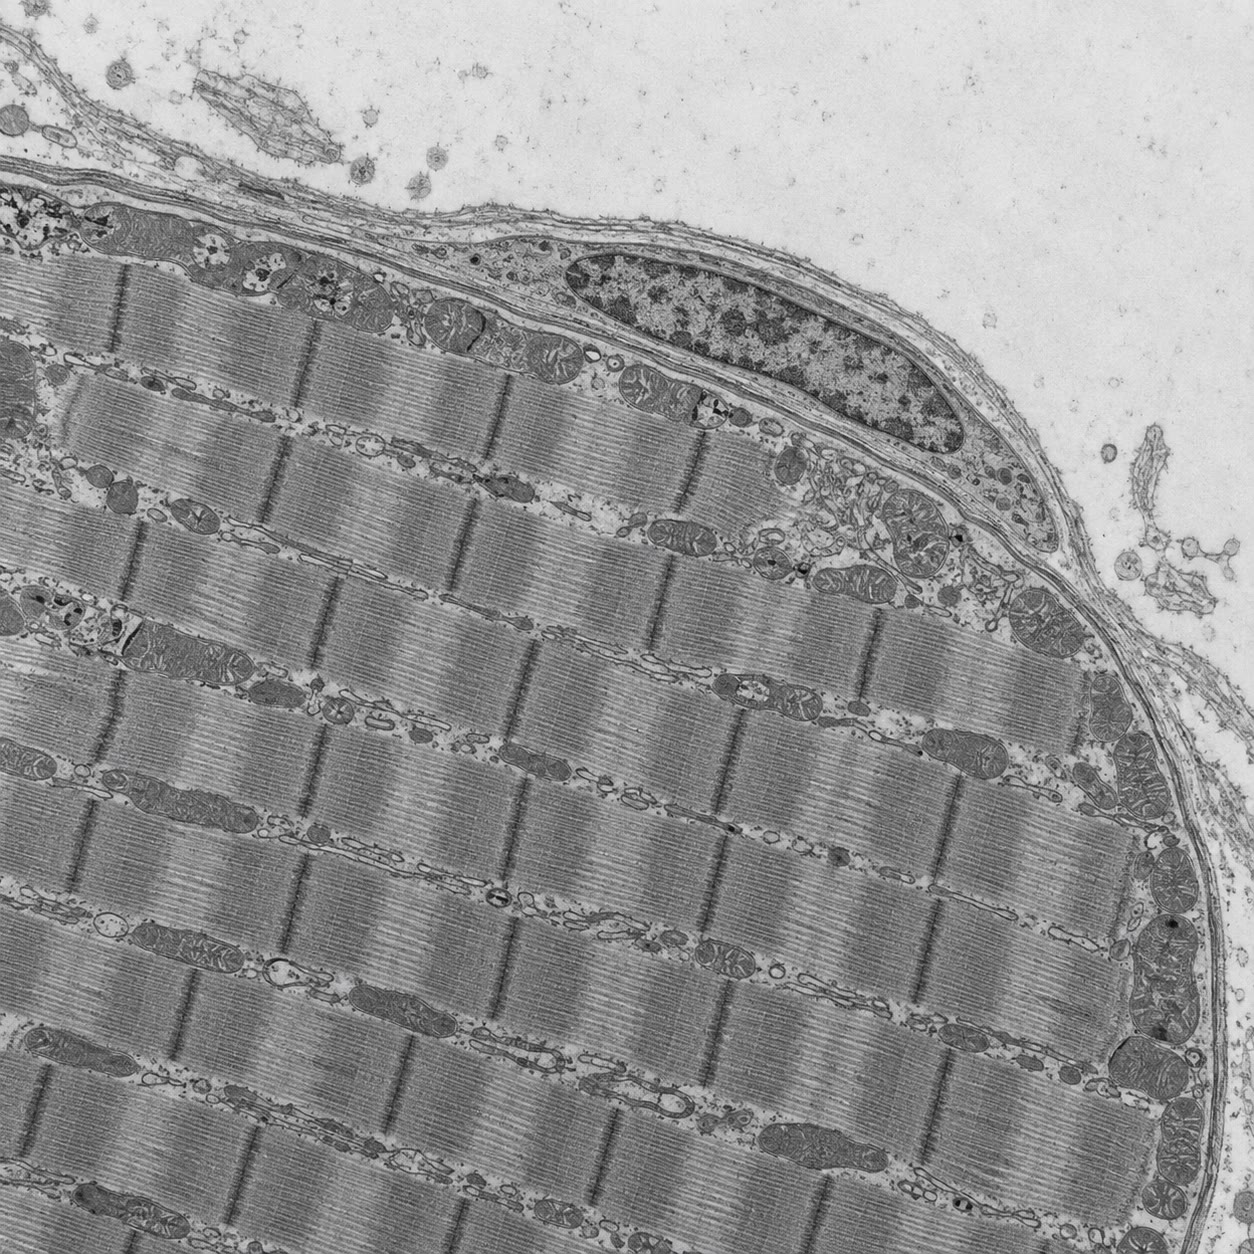
\includegraphics[width=0.42\linewidth]{images/book4/ai/b4-12-satellite-cell-tem.jpg}

{\small Uma célula satélite ao microscópio eletrônico: uma pequena
célula mononucleada encaixada entre a membrana de uma \omterm{def:b2:cell-differentiation:myogenesis}{fibra muscular} e
sua lâmina basal --- a reserva de \omterm{def:b2:cell-differentiation:myogenesis}{mioblastos} da fibra.}
\end{omfigure}

\section{Exercícios}

\begin{exercise}[$\star$]\label{exo:b2:cell-differentiation:1}
Defina \omterm{def:b2:cell-differentiation:differentiation}{diferenciação}, \omterm{def:b2:cell-differentiation:differentiation}{determinação} e \omterm{def:b2:cell-differentiation:differentiation}{potência}, e situe o zigoto, uma
célula da \omterm{def:b2:mammal-reproduction:implantation}{massa celular interna}, uma célula satélite e uma \omterm{def:b2:cell-differentiation:myogenesis}{fibra
muscular} na escala de \omterm{def:b2:cell-differentiation:differentiation}{potência}.
\end{exercise}

\begin{exercise}[$\star$]\label{exo:b2:cell-differentiation:2}
Liste as etapas da miogênese, da célula do somito à \omterm{def:b2:cell-differentiation:myogenesis}{fibra muscular}, com
o \omterm{prop:b2:cell-differentiation:transcriptional}{fator de transcrição} expresso em cada uma.
\end{exercise}

\begin{exercise}[$\star$]\label{exo:b2:cell-differentiation:3}
O que mostrou a transferência nuclear de Gurdon, e o que ela não mostrou?
\end{exercise}

\begin{exercise}[$\star$]\label{exo:b2:cell-differentiation:4}
Cite as partes de um \omterm{def:b2:cell-differentiation:fibre}{sarcômero} e diga quais se movem e quais não se
movem quando a fibra encurta.
\end{exercise}

\begin{exercise}[$\star\star$]\label{exo:b2:cell-differentiation:5}
Uma fibra de \qty{20}{cm} de comprimento tem \omterm{def:b2:cell-differentiation:fibre}{sarcômeros} de
\qty{2.5}{\micro m} e um núcleo a cada \qty{25}{\micro m} ao longo de
seu comprimento. Quantos \omterm{def:b2:cell-differentiation:fibre}{sarcômeros} em série, e quantos núcleos?
Quantos \omterm{def:b2:cell-differentiation:myogenesis}{mioblastos} se fundiram para formá-la?
\end{exercise}

\begin{exercise}[$\star\star$]\label{exo:b2:cell-differentiation:6}
Explique por que os \omterm{def:b2:cell-differentiation:myogenesis}{mioblastos} não se fundem enquanto há FGF, usando o
inibidor Id, e preveja o que acontece com \omterm{def:b2:cell-differentiation:myogenesis}{mioblastos} modificados para
produzir Id de forma constitutiva.
\end{exercise}

\begin{exercise}[$\star\star$]\label{exo:b2:cell-differentiation:7}
No modelo do interruptor com $a = 1$, $K = 1$, $b = 0.02$ e $k = 0.4$,
verifique por substituição que $m = 2.1$ está perto de um estado
estacionário, encontre aproximadamente o estado estacionário baixo e
diga o que acontece com uma célula cujo $m$ é elevado brevemente a $1$
e depois deixado livre.
\end{exercise}

\begin{exercise}[$\star\star$]\label{exo:b2:cell-differentiation:8}
No mesmo modelo, $k$ é elevado a $0.6$ (o fator é degradado mais
depressa). Mostre gráfica ou numericamente que o estado alto
desaparece. O que isso prevê para uma célula em que a \omterm{def:b2:cell-differentiation:myogenesis}{MyoD} é
desestabilizada?
\end{exercise}

\begin{exercise}[$\star\star$]\label{exo:b2:cell-differentiation:9}
Preveja o \omterm{def:b2:meiosis-heredity:vocabulary}{fenótipo} de um camundongo sem (a) \omterm{def:b2:cell-differentiation:myogenesis}{MyoD} e Myf5, (b) apenas
miogenina, (c) apenas \omterm{def:b2:cell-differentiation:myogenesis}{MyoD}. Por que (c) é quase normal?
\end{exercise}

\begin{exercise}[$\star\star\star$]\label{exo:b2:cell-differentiation:10}
Um fibroblasto transfectado com \omterm{def:b2:cell-differentiation:myogenesis}{MyoD} se torna um \omterm{def:b2:cell-differentiation:myogenesis}{miotubo}; uma célula
hepática transfectada com \omterm{def:b2:cell-differentiation:myogenesis}{MyoD}, não. Proponha uma explicação que
envolva a cromatina e a \omterm{def:b2:vertebrate-development:induction}{competência}, e um experimento para testá-la.
\end{exercise}

\begin{exercise}[$\star\star\star$]\label{exo:b2:cell-differentiation:11}
O treino de resistência converte fibras rápidas para o tipo lento sem
mudar seu genoma. Explique, em termos de expressão gênica, como o
padrão de disparos do nervo pode fazer isso, e por que as fibras,
apesar disso, continuam sendo músculo esquelético e nunca se tornam,
digamos, cartilagem.
\end{exercise}

\begin{exercise}[$\star\star\star$]\label{exo:b2:cell-differentiation:12}
``Uma célula diferenciada lembra o que ela é com um circuito, e não com
uma \omterm{def:b2:genome-diversification:mutation}{mutação}.'' Discuta, com o interruptor biestável, a cromatina e o
fato de que as reinicializações de Gurdon e de Yamanaka são possíveis,
mas pouco eficientes.
\end{exercise}

\section{Problema: Um músculo construído e reconstruído}

\begin{problem}[{Problema de fim de semana --- um músculo acompanhado
do somito à fibra e através de uma lesão: os números de mioblastos, de
fusões e de núcleos, o interruptor biestável analisado, um reparo
cronometrado e o treino quantificado, até o número de núcleos da fibra,
o limiar do interruptor e o tempo de reparo}]
\label{pb:b2:cell-differentiation:1}
Um músculo da coxa de um adulto tem \num{500000} fibras, cada uma com
\qty{20}{cm} de comprimento e \qty{60}{\micro m} de diâmetro, com um
núcleo por \qty{25}{\micro m} de comprimento; os \omterm{def:b2:cell-differentiation:fibre}{sarcômeros} têm
\qty{2.5}{\micro m}. Os \omterm{def:b2:cell-differentiation:myogenesis}{mioblastos} embrionários se dividem a cada
\qty{12}{h} enquanto há FGF. Modelo do interruptor: $a = 1$, $K = 1$,
$b = 0.02$, $k
= 0.4$. Após uma lesão que destrói \qty{10}{\%} do comprimento de cada
fibra, as células satélites do segmento lesado (\num{4} por milímetro
de fibra) se dividem a cada \qty{18}{h} durante algum tempo e depois
se fundem.

\medskip
\noindent\textbf{Parte I --- A fibra.}
\begin{enumerate}
  \item Calcule o número de \omterm{def:b2:cell-differentiation:fibre}{sarcômeros} em série numa fibra e o número de
        núcleos.
  \item Quantos \omterm{def:b2:cell-differentiation:myogenesis}{mioblastos} se fundiram para formar uma fibra? E o
        músculo inteiro?
  \item Calcule o volume de uma fibra e o do músculo (em litros).
  \item Estime o volume de citoplasma servido por um núcleo, e compare
        com uma célula comum de \qty{2000}{\micro m^3}.
  \item Por que os núcleos ficam na periferia de uma fibra madura?
  \item Os \omterm{def:b2:cell-differentiation:myogenesis}{mioblastos} do músculo descendem de \num{2000} células do
        somito. Quantas duplicações foram necessárias, e quantos dias,
        para chegar ao número da questão 2?
\end{enumerate}

\medskip
\noindent\textbf{Parte II --- O interruptor.}
\begin{enumerate}[resume]
  \item Escreva a condição de estado estacionário e mostre que
        $m \approx
        0.055$ a satisfaz.
  \item Mostre que $m \approx 2.1$ a satisfaz.
  \item Mostre que há uma terceira solução perto de $m = 0.41$, e
        explique, pelos sinais de $\mathrm{d}m/\mathrm{d}t$ de cada lado,
        que ela é instável.
  \item Um pulso de indutor eleva $m$ a $0.6$; outro, a $0.3$. Qual é o
        destino de cada célula?
  \item A síntese basal $b$ é elevada a $0.4$ por uma \omterm{def:b2:genome-diversification:mutation}{mutação}. Mostre
        que o estado baixo desaparece. O que a célula faz?
  \item Explique como esse modelo dá conta de um comprometimento que
        sobrevive à divisão celular, e o que precisa ser verdade sobre
        $m$ a cada divisão.
\end{enumerate}

\medskip
\noindent\textbf{Parte III --- O reparo.}
\begin{enumerate}[resume]
  \item Quantas células satélites uma fibra tem, e quantos núcleos
        precisam ser substituídos após a lesão?
  \item Quantas duplicações as células satélites precisam fazer para
        fornecê-los, e quanto tempo isso leva?
  \item Compare com as duas a três semanas observadas para o reparo, e
        diga o que mais esse tempo inclui.
  \item Por que as células satélites precisam voltar a expressar \omterm{def:b2:cell-differentiation:myogenesis}{MyoD}
        antes de se fundir, e por que precisam parar de se dividir
        antes?
  \item Cada rodada de reparo consome algumas células satélites. Se o
        estoque cai \qty{5}{\%} por lesão, quantas lesões até que ele
        caia à metade?
  \item Quantas células satélites por fibra restam após vinte lesões
        desse tipo?
  \item Explique por que um músculo distrófico, cujas fibras se rompem
        a cada contração, é substituído por tecido fibroso após anos.
\end{enumerate}

\medskip
\noindent\textbf{Parte IV --- O treino.}
\begin{enumerate}[resume]
  \item O treino engrossa cada fibra para \qty{80}{\micro m}. Por que
        fator cresce o volume da fibra, e quantos núcleos adicionais as
        células satélites precisam fornecer se a razão da questão 4 for
        mantida?
  \item Calcule o novo volume do músculo.
  \item O treino de resistência converte \qty{30}{\%} das fibras
        rápidas em lentas. O que mudou nessas fibras, e o que não mudou?
  \item Explique por que um músculo adulto aumenta pelo crescimento das
        fibras, e não pela adição de fibras, usando o fato de que as
        fibras não se dividem.
  \item Um fármaco bloqueia a fusão das células satélites. Preveja a
        resposta do músculo ao treino e à lesão.
  \item Enuncie o resultado: o número de núcleos da fibra, o limiar do
        interruptor e o tempo para que as células satélites forneçam os
        núcleos de um reparo.
\end{enumerate}
\end{problem}
